%
% 2d_basisfkt.tex
%
% (c) 2024 Flurin Brechbühler
%
\begin{figure}
    \centering
    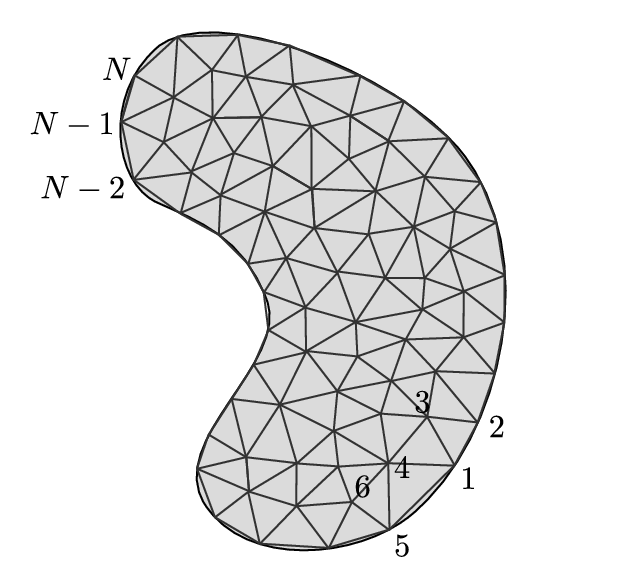
\includegraphics[width=0.45\textwidth]{papers/fem/images/2d_mesh.png}
    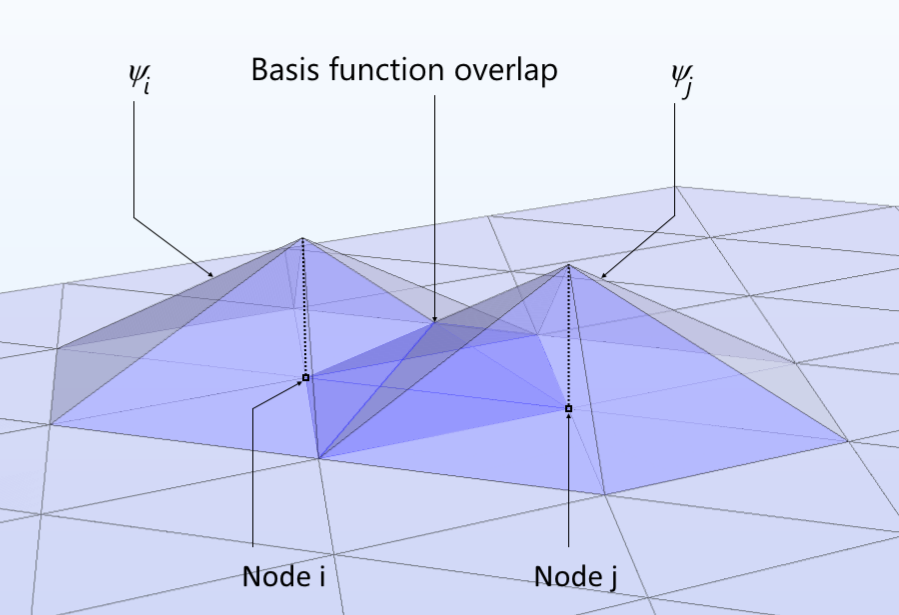
\includegraphics[width=0.45\textwidth]{papers/fem/images/2d_basisfkt.png}
    \caption{Der in dreieckige Elemente unterteilte Definitionsbereich mit nummerierten Knotenpunkten (links) und die linearen Basisfunktionen zweier Elemente, die sich berühren.}
    \label{fem:nd:2d_mesh_und_basisfkt}
    \end{figure}
    